\section{实验结果}

\subsection{实验数据记录及处理}

\subsubsection{确定旋光仪的零点}

重复测量旋光仪零点 5 次,数据示于表 \ref{tab:1}。
 
\begin{table}[htbp]
    \centering
    \bicaption{旋光仪零点测量数据}{Polarimeter zero point measurement data}
    \begin{tabular}{c|ccccc}
        \toprule
        编号 & 1 & 2 & 3 & 4 & 5  \\
        \midrule
        $\alpha_0$ / ${}^{\circ}$ & 0.00 & 0.05 & 0.00 & 0.00 & -0.05\\
        \bottomrule
    \end{tabular}
    \label{tab:1}
\end{table}

根据表 \ref{tab:1} 数据,计算旋光仪零点的平均值为
\begin{equation*}
    \alpha_0=0.00^\circ
\end{equation*}
$\alpha_0$的标准偏差
\begin{equation*}
    \sigma_{\alpha_0} = 0.04^\circ
\end{equation*}

故旋光仪零点为
\begin{equation*}
    \alpha=(0.00 \pm 0.04)^{\circ}
\end{equation*}

\subsubsection{旋光度的测定}

依次测定 $6.16 \mathrm{~M} $、$ 4.19 \mathrm{~M} $、$ 3.12 \mathrm{~M} $ 的盐酸溶液与蔗糖溶液的混合液不同时间 $t$ 时的旋光度 $\alpha_t$ 。由于第 1 次测定 $6.16 \mathrm{M}$ 的盐酸溶液与蔗糖溶液的混合液的旋光度变化时,恒温水水管联通不畅进入气泡,导致半途恒温水停止流动,使得数据不够可靠,故重新测定了一组 $6.16 \mathrm{M}$ 的盐酸溶液与蔗糖溶液的混合液的旋光度。

记实验测得原始旋光角为 $\alpha_t^{\prime}$,根据
$$
\alpha_t=\alpha_t^{\prime}-\alpha
$$

处理原始数据,原始旋光角 $\alpha_t^{\prime}$ 减去旋光仪的零点 $\alpha$,得到实际的旋光角 $\alpha_t$ 。 以上各项数据示于表 \ref{tab:2}。

\begin{table}[H]
    \centering
    \bicaption{不同盐酸浓度下混合液 $t-\alpha_t$ 测量数据}{Measurement data of $t-\alpha_t$ under different hydrochloric acid concentration}
    \begin{tabular}{ccc|ccc|ccc}
        \toprule
        \multicolumn{3}{c|}{6.16 M HCl} & \multicolumn{3}{c|}{4.19 M HCl} & \multicolumn{3}{c}{3.12 M HCl} \\
        \midrule
        $t/ \mathrm{s}$ & $\alpha_t^{\prime}/^{\circ}$ & $\alpha_t/^{\circ}$ & $t/ \mathrm{s}$ & $\alpha_t^{\prime}/^{\circ}$ & $\alpha_t/^{\circ}$ & $t/ \mathrm{s}$ & $\alpha_t^{\prime}/^{\circ}$ & $\alpha_t/^{\circ}$ \\
        \midrule
        201 & 4.20 & 4.20 & 155 & 8.80 & 8.80 & 181 & 11.95 & 11.95 \\
        234 & 3.60 & 3.60 & 186 & 8.50 & 8.50 & 231 & 10.55 & 10.55 \\
        261 & 3.20 & 3.20 & 215 & 8.35 & 8.35 & 268 & 9.80 & 9.80 \\
        290 & 2.80 & 2.80 & 240 & 7.95 & 7.95 & 311 & 9.35 & 9.35 \\
        308 & 2.30 & 2.30 & 266 & 7.40 & 7.40 & 349 & 8.90 & 8.90 \\
        332 & 1.80 & 1.80 & 296 & 7.10 & 7.10 & 383 & 8.15 & 8.15 \\
        368 & 1.40 & 1.40 & 319 & 6.90 & 6.90 & 418 & 7.70 & 7.70 \\
        396 & 0.90 & 0.90 & 353 & 6.20 & 6.20 & 458 & 7.20 & 7.20 \\
        426 & 0.20 & 0.20 & 382 & 5.55 & 5.55 & 499 & 6.90 & 6.90 \\
        456 & -0.05 & -0.05 & 415 & 5.30 & 5.30 & 554 & 6.50 & 6.50 \\
        484 & -0.20 & -0.20 & 458 & 5.00 & 5.00 & 601 & 5.85 & 5.85 \\
        520 & -0.55 & -0.55 & 489 & 4.70 & 4.70 & 645 & 5.50 & 5.50 \\
        562 & -0.90 & -0.90 & 510 & 4.25 & 4.25 & 711 & 5.05 & 5.05 \\
        583 & -1.05 & -1.05 & 536 & 4.10 & 4.10 & 767 & 4.75 & 4.75 \\
        614 & -1.35 & -1.35 & 567 & 3.65 & 3.65 & 826 & 4.60 & 4.60 \\
        637 & -1.75 & -1.75 & 622 & 3.15 & 3.15 & 904 & 4.10 & 4.10 \\
        659 & -1.80 & -1.80 & 674 & 3.00 & 3.00 & 955 & 3.60 & 3.60 \\
        677 & -1.90 & -1.90 & 712 & 2.75 & 2.75 & 1023 & 3.20 & 3.20 \\
        705 & -2.00 & -2.00 & 739 & 2.55 & 2.55 & 1094 & 2.60 & 2.60 \\
        724 & -2.15 & -2.15 & 780 & 2.00 & 2.00 & 1148 & 2.30 & 2.30 \\
        752 & -2.35 & -2.35 & 818 & 1.60 & 1.60 & 1215 & 2.05 & 2.05 \\
        827 & -2.70 & -2.70 & 865 & 1.30 & 1.30 & 1317 & 1.70 & 1.70 \\
        \multicolumn{3}{c|}{\multirow{7}{*}{}} & 948 & 0.55 & 0.55 & 1438 & 1.40 & 1.40 \\
        \multicolumn{3}{c|}{} & 1031 & -0.15 & -0.15 & 1530 & 1.00 & 1.00 \\
        \multicolumn{3}{c|}{} & \multicolumn{3}{c|}{\multirow{5}{*}{}} & 1660 & 0.50 & 0.50 \\
        \multicolumn{3}{c|}{} & \multicolumn{3}{c|}{} & 1761 & 0.00 & 0.00 \\
        \multicolumn{3}{c|}{} & \multicolumn{3}{c|}{} & 1870 & -0.10 & -0.10 \\
        \multicolumn{3}{c|}{} & \multicolumn{3}{c|}{} & 1898 & -0.13 & -0.13 \\
        \bottomrule
    \end{tabular}
    \label{tab:2}
\end{table}

\subsubsection{$\alpha_{\infty}$ 的测定}

测量保留备用的两次测定时的 $6.16 \mathrm{M}$ 盐酸溶液与蔗糖溶液的混合液的旋光度,重复测量 5 次,读取旋光仪的原始旋光角 $\alpha_{\infty}^{\prime}$,根据
\begin{equation}\label{eq:1}
    \alpha_{\infty}=\alpha_{\infty}^{\prime}-\alpha_0
\end{equation}
处理原始数据,得到实际的 $\alpha_{\infty}$ 。各项数据示于表 \ref{tab:3}。

\begin{table}[htbp]
\centering
\bicaption{$\alpha_{\infty}$ 测量数据}{Table $3 \alpha_{\infty}$ measurement data}
\begin{tabular}{c|ccccc|ccccc}
\toprule
\multirow{2}{*}{编号} & \multicolumn{5}{c|}{溶液1} & \multicolumn{5}{c}{溶液2} \\
 & 1 & 2 & 3 & 4 & 5 & 1 & 2 & 3 & 4 & 5 \\
\midrule
$\alpha_{\infty}^{\prime} /{ }^{\circ}$ & -4.05 & -4.05 & -4.08 & -4.05 & -4.00 & -3.98 & -4.00 & -4.02 & -4.05 & -3.95 \\
$\alpha_{\infty} /{ }^{\circ}$ & -4.05 & -4.05 & -4.08 & -4.05 & -4.00 & -3.98 & -4.00 & -4.02 & -4.05 & -3.95 \\
\bottomrule
\end{tabular}
\label{tab:3}
\end{table}

根据表 3 数据,计算 $\alpha_{\infty}$ 的平均值为
$$
\alpha_{\infty} = -4.02^{\circ}
$$
$\alpha_{\infty}$ 的标准差为
$$
s_{\alpha_{\infty}} = 0.04^{\circ}
$$
根据公式 \eqref{eq:1},$\alpha_{\infty}$ 的误差为
$$
\sigma_{\alpha_{\infty}} = \sqrt{s_{\alpha_{\infty}}^2+\sigma_{\alpha_0}^2}=0.06^{\circ}
$$

故 $\alpha_{\infty}$ 测定值为
$$
\alpha_{\infty} = −(4.02 \pm 0.06)^{\circ}
$$

\subsection{数据处理结果与分析}

\subsubsection{$\alpha_t-t$ 图的绘制}

根据表 \ref{tab:2} 数据,使用python matplotlab,作出不同盐酸浓度下混合液 $\alpha_t-t$ 图,如图 \ref{fig:1} 所示。

\begin{figure}[htbp]
    \centering
    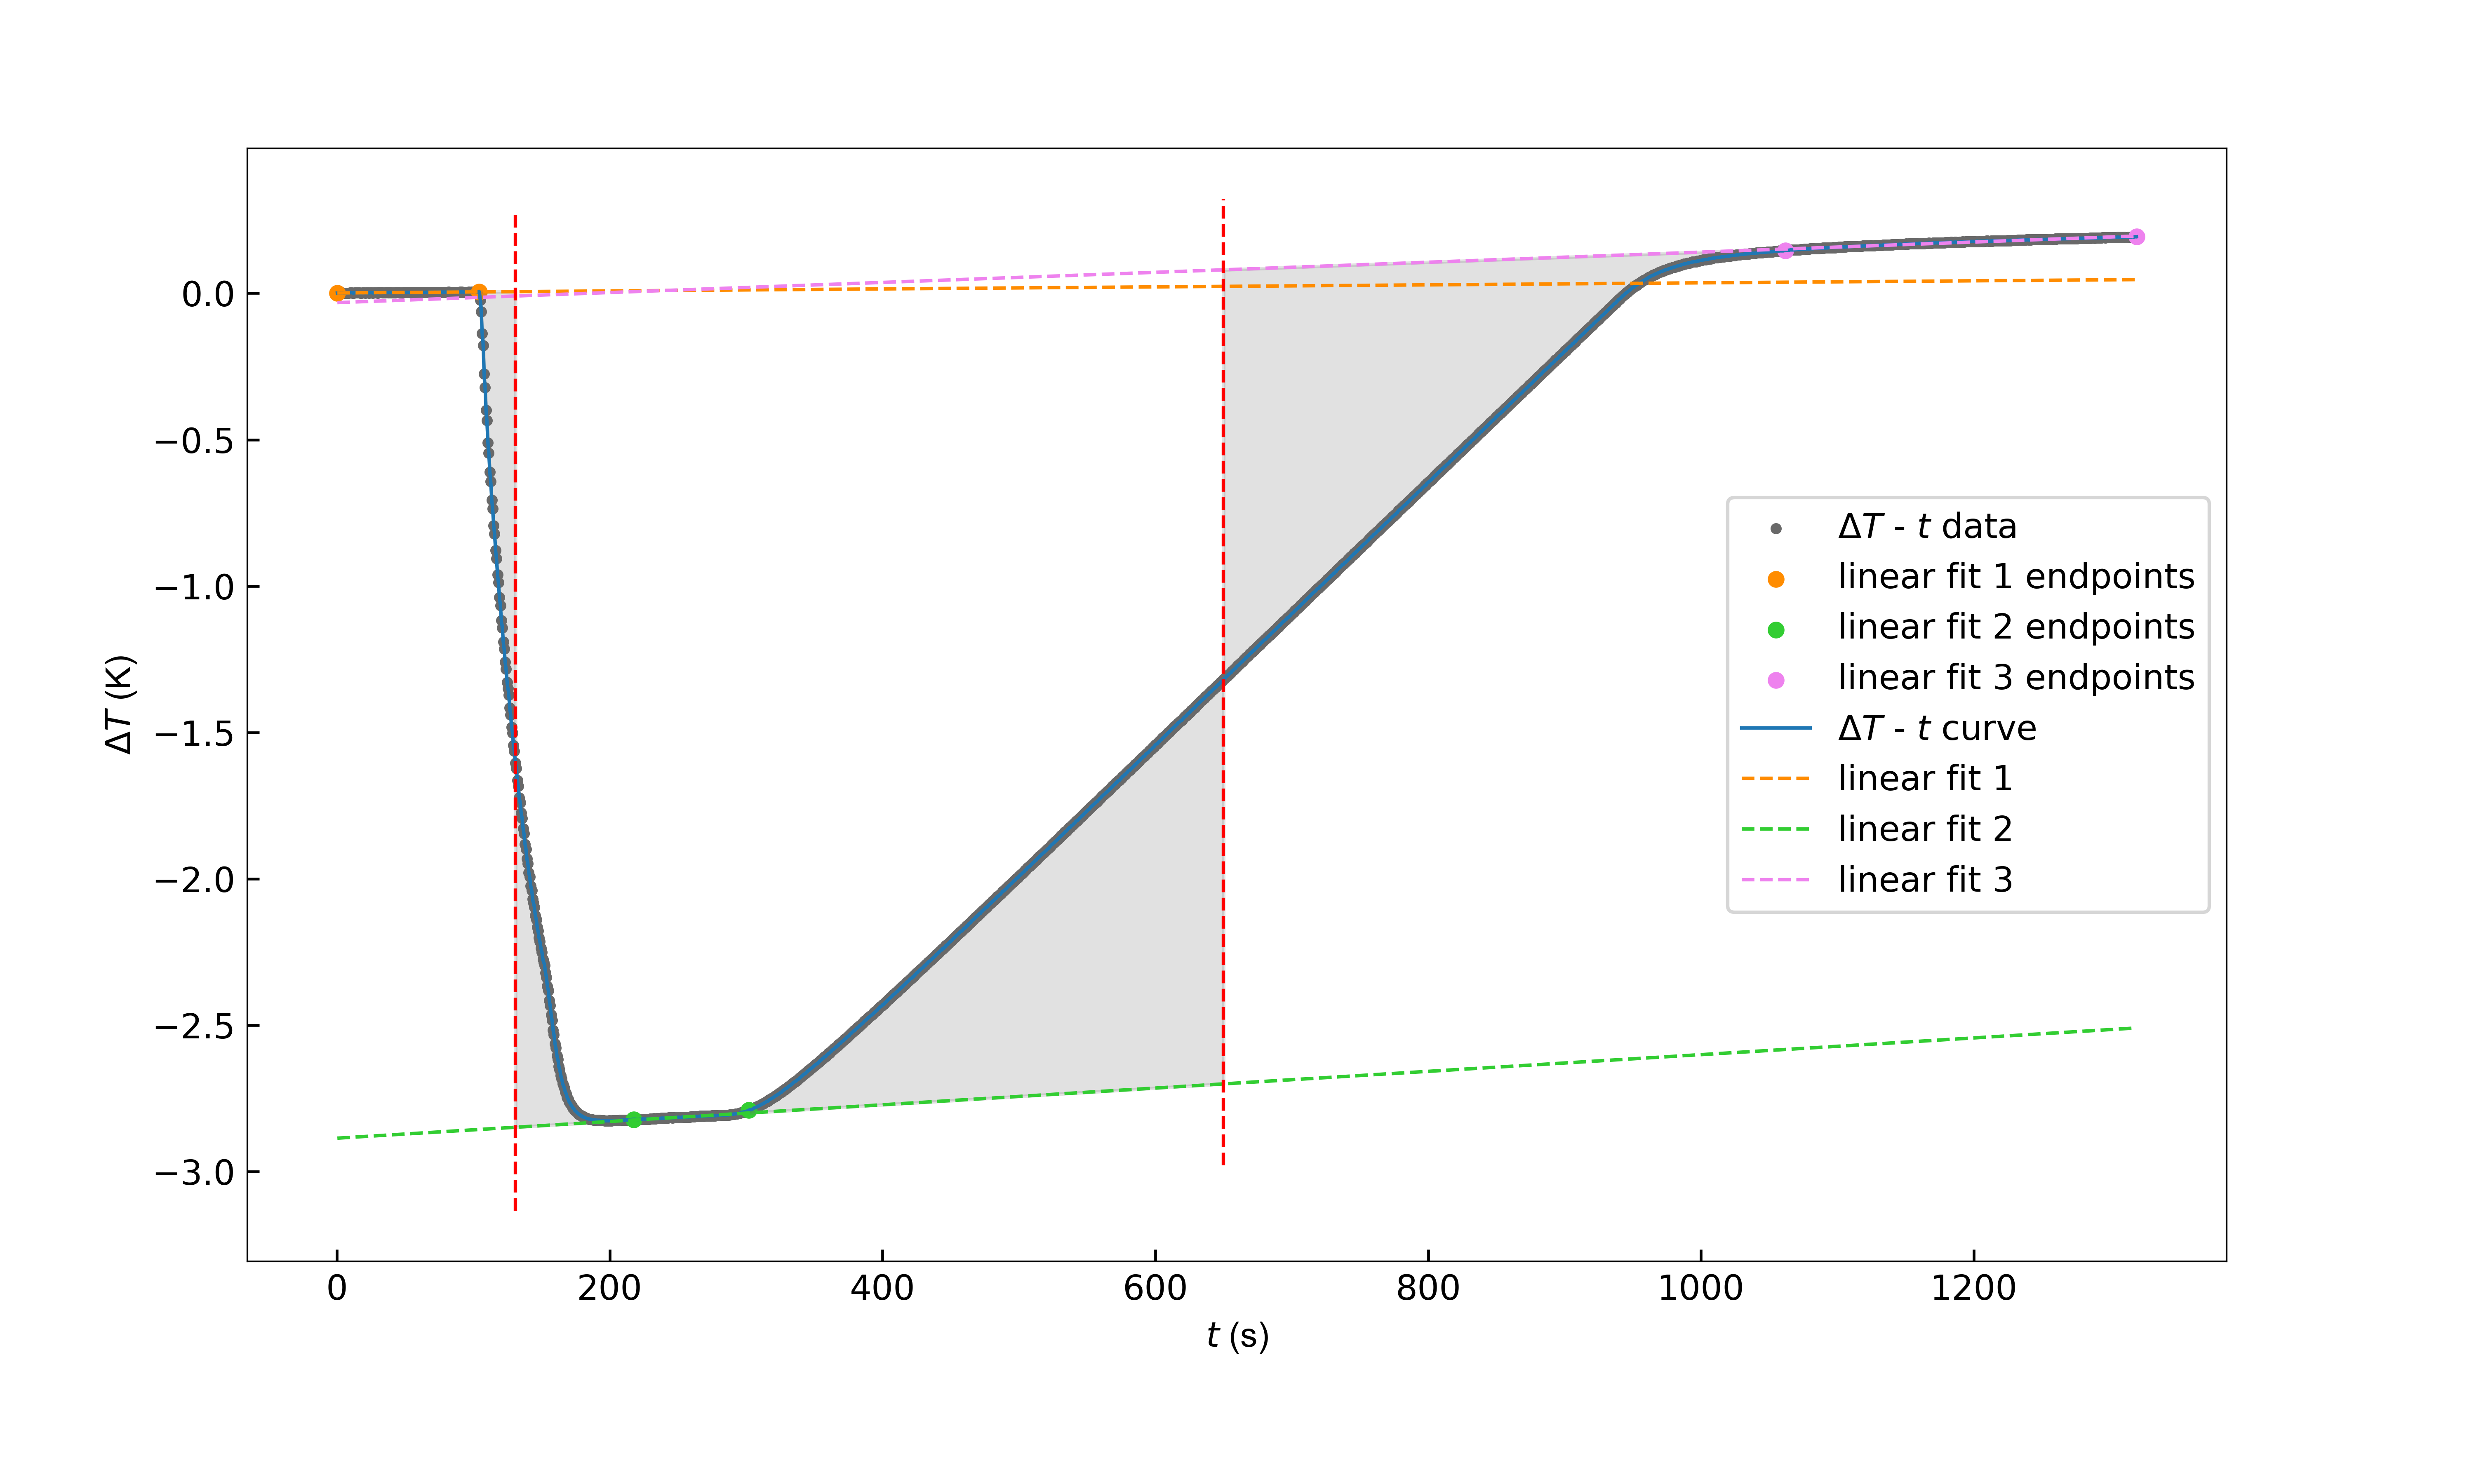
\includegraphics[width=.8\textwidth]{figures/1.png}
    \bicaption{不同盐酸浓度下混合液 $\alpha_t-t$ 图}{$\alpha_t-t$ diagram under different hydrochloric acid concentration}
    \label{fig:1}
\end{figure}

在图 \ref{fig:1} 中,标出的盐酸浓度为加入的盐酸溶液的浓度,与蔗糖溶液混合后实际的盐酸浓度为该数值的一半。根据图 \ref{fig:1} 可以看出,同一时间 $\alpha_t$ 随盐酸浓度增大而减小,即随着盐酸度升高,蔗糖转化反应速度加快。

\subsubsection{$\left(\alpha_t-\alpha_{\infty}\right)$ 和 $\lg \left(\alpha_t-\alpha_{\infty}\right)$ 的数据处理}

根据表 \ref{tab:2} 数据和 $\alpha_{\infty}=-4.02^{\circ}$,计算不同盐酸浓度下的 $\left(\alpha_t-\alpha_{\infty}\right)$ 和 $\lg \left(\alpha_t-\alpha_{\infty}\right)$ 数据,记$\alpha^\prime = \left(\alpha_t-\alpha_{\infty}\right)$,计算得到各项数据示于表 \ref{tab:4}。

\begin{table}[H]
    \centering
    \bicaption{不同盐酸浓度下混合液 $\left(\alpha_t-\alpha_{\infty}\right)$ 和 $\lg \left(\alpha_t-\alpha_{\infty}\right)$ 数据}{Data of $\left(\alpha_t-\alpha_{\infty}\right)$ 和 $\lg \left(\alpha_t-\alpha_{\infty}\right)$ under different hydrochloric acid concentration}
    \begin{tabular}{ccc|ccc|ccc}
        \toprule
        \multicolumn{3}{c|}{6.16 M HCl} & \multicolumn{3}{c|}{4.19 M HCl} & \multicolumn{3}{c}{3.12 M HCl} \\
       $t$/s & $\alpha^\prime/\mathrm{{}^\circ}$ & $\lg \left[(\alpha^\prime)/\mathrm{{}^\circ}\right]$ & $t$/s & $\alpha^\prime/\mathrm{{}^\circ}$ & $\lg \left[(\alpha^\prime)/\mathrm{{}^\circ}\right]$ & $t$/s & $\alpha^\prime/\mathrm{{}^\circ}$ & $\lg \left[(\alpha^\prime)/\mathrm{{}^\circ}\right]$ \\
        \midrule
        201 & 8.22 & 0.915 & 155 & 12.82 & 1.108 & 181 & 15.97 & 1.203 \\
        234 & 7.62 & 0.882 & 186 & 12.52 & 1.098 & 231 & 14.57 & 1.164 \\
        261 & 7.22 & 0.859 & 215 & 12.37 & 1.092 & 268 & 13.82 & 1.141 \\
        290 & 6.82 & 0.834 & 240 & 11.97 & 1.078 & 311 & 13.37 & 1.126 \\
        308 & 6.32 & 0.801 & 266 & 11.42 & 1.058 & 349 & 12.92 & 1.111 \\
        332 & 5.82 & 0.765 & 296 & 11.12 & 1.046 & 383 & 12.17 & 1.085 \\
        368 & 5.42 & 0.734 & 319 & 10.92 & 1.038 & 418 & 11.72 & 1.069 \\
        396 & 4.92 & 0.692 & 353 & 10.22 & 1.010 & 458 & 11.22 & 1.050 \\
        426 & 4.22 & 0.626 & 382 & 9.57 & 0.981 & 499 & 10.92 & 1.038 \\
        456 & 3.97 & 0.599 & 415 & 9.32 & 0.970 & 554 & 10.52 & 1.022 \\
        484 & 3.82 & 0.582 & 458 & 9.02 & 0.955 & 601 & 9.87 & 0.994 \\
        520 & 3.47 & 0.541 & 489 & 8.72 & 0.941 & 645 & 9.52 & 0.979 \\
        562 & 3.12 & 0.495 & 510 & 8.27 & 0.918 & 711 & 9.07 & 0.958 \\
        583 & 2.97 & 0.473 & 536 & 8.12 & 0.910 & 767 & 8.77 & 0.943 \\
        614 & 2.67 & 0.427 & 567 & 7.67 & 0.885 & 826 & 8.62 & 0.936 \\
        637 & 2.27 & 0.357 & 622 & 7.17 & 0.856 & 904 & 8.12 & 0.910 \\
        659 & 2.22 & 0.347 & 674 & 7.02 & 0.847 & 955 & 7.62 & 0.882 \\
        677 & 2.12 & 0.327 & 712 & 6.77 & 0.831 & 1023 & 7.22 & 0.859 \\
        705 & 2.02 & 0.306 & 739 & 6.57 & 0.818 & 1094 & 6.62 & 0.821 \\
        724 & 1.87 & 0.273 & 780 & 6.02 & 0.780 & 1148 & 6.32 & 0.801 \\
        752 & 1.67 & 0.223 & 818 & 5.62 & 0.750 & 1215 & 6.07 & 0.783 \\
        827 & 1.32 & 0.122 & 865 & 5.32 & 0.726 & 1317 & 5.72 & 0.758 \\
        \multicolumn{3}{c|}{\multirow{2}{*}{}} & 948 & 4.57 & 0.660 & 1438 & 5.42 & 0.734 \\
        \multicolumn{3}{c|}{} & 1031 & 3.87 & 0.588 & 1530 & 5.02 & 0.701 \\
        \multicolumn{3}{c|}{\multirow{4}{*}{}} & \multicolumn{3}{c|}{\multirow{4}{*}{}} & 1660 & 4.52 & 0.655 \\
        \multicolumn{3}{c|}{} & \multicolumn{3}{c|}{} & 1761 & 4.02 & 0.605 \\
        \multicolumn{3}{c|}{} & \multicolumn{3}{c|}{} & 1870 & 3.92 & 0.594 \\
        \multicolumn{3}{c|}{} & \multicolumn{3}{c|}{} & 1898 & 3.89 & 0.590 \\
        \bottomrule
        \end{tabular}
    \label{tab:4}
\end{table}

\subsubsection{$\lg \left(\alpha_t-\alpha_{\infty}\right)-t$ 图与反应级数}

根据表 \ref{tab:4} 数据,作出不同盐酸浓度下混合液 $\lg \left(\alpha_t-\alpha_{\infty}\right)-t$ 散点图,并用 python处理数据:使用scipy.stats.linregress() 进行线性拟合参数与相关系数的计算,使用scipy.optimize.curve\_fit() 计算线性拟合的参数误差。作出不同盐酸浓度下混合液 $\lg \left(\alpha_t-\alpha_{\infty}\right)-t$ 拟合直线,如图 \ref{fig:2} 所示。根据图 \ref{fig:2} 可以看出,不同盐酸浓度下 $\lg \left(\alpha_t-\alpha_{\infty}\right)-t$ 都具有良好的线性关系,根据一级反应的动力学特征
$$
\ln \frac{c_0}{c_t}=k t
$$

可以判断 \ce{H+} 浓度固定的条件下,蔗糖转化反应为一级反应。 6.16 M、4.15 M、3.12 M 盐酸浓度下的回归直线方程分别为:
\begin{align*}
     &\lg \left[(\alpha_t-\alpha_{\infty})/{}^\circ\right] = (-1.27 \pm 0.02) \times 10^{-3}t/\si{s} + (1.19 \pm 0.01);\quad &R^2 = 0.99654 \\
     &\lg \left[(\alpha_t-\alpha_{\infty})/{}^\circ\right] = (-5.68 \pm 0.11) \times 10^{-4}t/\si{s} + (1.21 \pm 0.01);\quad &R^2 = 0.99154 \\
     &\lg \left[(\alpha_t-\alpha_{\infty})/{}^\circ\right] = (-3.46 \pm 0.06) \times 10^{-4}t/\si{s} + (1.22 \pm 0.01);\quad &R^2 = 0.99192
\end{align*}

\begin{figure}[htbp]
    \centering
    \includegraphics[width=.8\textwidth]{figures/2.png}
    \bicaption{不同盐酸浓度下混合液 $\lg \left(\alpha_t-\alpha_{\infty}\right)-t$ 图}{$\lg \left(\alpha_t-\alpha_{\infty}\right)-t$ diagram under different hydrochloric acid concentration}
    \label{fig:2}
\end{figure}

根据
$$
\lg \left(\alpha_t-\alpha_{\infty}\right)=-\frac{k}{2.303} t+\lg \left(\alpha_0-\alpha_{\infty}\right)
$$
可以用拟合直线的斜率 $a$ 计算速率常数 $k$,即
$$
k=-2.303 a
$$
显然,速率常数的误差
$$
\sigma_k=2.303 \sigma_a
$$

对于一级反应,其半衰期$t_{1/2}$
$$
t_{1 / 2}=\frac{\ln 2}{k}=\frac{0.693}{k}
$$
半衰期的误差
$$
\sigma_{t_{1 / 2}}=\ln 2 \frac{\sigma_k}{k^2}=0.693 \frac{\sigma_k}{k^2}
$$

根据拟合直线方程,计算不同盐酸浓度下的反应速率常数 $k$ 、半衰期 $t_{1 / 2}$ 及各自的标准差 $\sigma_k $、$ \sigma_{t_{1 / 2}}$,结果示于表 \ref{tab:5},其中 $c(\ce{HCl})$ 是加入盐酸的浓度,$a$ 是拟合直线的斜率。

\begin{table}[htbp]
    \centering
    \bicaption{不同盐酸浓度下 $k$ 与 $t_{1 / 2}$ 计算结果}{Calculation results of $k$ and $t_{1 / 2}$ under different hydrochloric acid concentrations}
    \begin{tabular}{cccc}
    \toprule
         $c(\ce{HCl}) / \mathrm{M}$ & $a /\mathrm{~s}^{-1}$ & $k /\mathrm{~s}^{-1}$ & $t_{1 / 2} / \mathrm{s}$\\
         \midrule
        6.16 & $(-1.27 \pm 0.02) \times 10^{-3}$ & $(2.92 \pm 0.04) \times 10^{-3}$ & $(237 \pm 3) $ \\
        4.19 & $(-5.68 \pm 0.11) \times 10^{-4}$ & $(1.31 \pm 0.03) \times 10^{-3}$ & $(530 \pm 10) $ \\
        3.12 & $(-3.46 \pm 0.06) \times 10^{-4}$ & $(7.96 \pm 0.14) \times 10^{-4}$ & $(870 \pm 15) $ \\
    \bottomrule
    \end{tabular}
    \label{tab:5}
\end{table}

\subsubsection{\ce{H+} 的反应级数}

考虑 \ce{H+} 对反应速率的影响,有
$$
k=k_0+k_{\mathrm{H}^{+}} c_{\mathrm{H}^{+}}^n
$$
其中 $k_0$ 是 $c_{\mathrm{H}^{+}} \rightarrow 0$ 时的反应速率常数,$k_{\mathrm{H}^{+}}$为酸催化速率常数,$k$ 为表观速率常数,$n$ 为 $\mathrm{H}^{+}$的反应级数。由于蔗糖在水溶液中能够稳定存在,其在非催化条件下的自发水解速率很慢,因此,忽略 $k_0$ ,然后等式两边取以自然对数,即得
$$
\ln \left(k\right)=n \ln c_{\mathrm{H}^{+}}+\ln k_{\mathrm{H}^{+}}
$$

氢离子浓度和反应速率常数数据处理如表 \ref{tab:6}。根据表 \ref{tab:6} 中的数据作出 $\ln\left(k/\mathrm{M}^{-1}\right)-\ln\left([\mathrm{H}^+]/\mathrm{M}\right)$ 散点图,并用 python处理数据:使用scipy.stats.linregress() 进行线性拟合参数与相关系数的计算,使用scipy.optimize.curve\_fit() 计算线性拟合的参数误差,作出 $\ln\left(k/\mathrm{M}^{-1}\right)-\ln\left([\mathrm{H}^+]/\mathrm{M}\right)$  拟合直线,如图 \ref{fig:3} 所示。

\begin{table}[H]
    \centering
    \bicaption{$\ln ([\ce{H+}] / \si{M})$与 $\ln (k/\si{M^{-1}})$ 计算结果}{Calculation results of $\ln ([\ce{H+}] / \si{M})$ and $\ln (k/\si{M^{-1}})$}
    \begin{tabular}{cccc}
    \toprule
        $[\ce{H+}] / \si{M}$ & $\ln ([\ce{H+}] / \si{M})$ & $k/\si{M^{-1}}$ & $\ln (k/\si{M^{-1}})$ \\
        \midrule
        3.12 & 1.138 & $7.96\times 10^{-4}$ & -7.135 \\
        4.19 & 1.433 & $1.31\times 10^{-3}$ & -6.640 \\
        6.16 & 1.818 & $2.92\times 10^{-3}$ & -5.835 \\
        \bottomrule
    \end{tabular}
    \label{tab:6}
\end{table}

\begin{figure}[H]
    \centering
    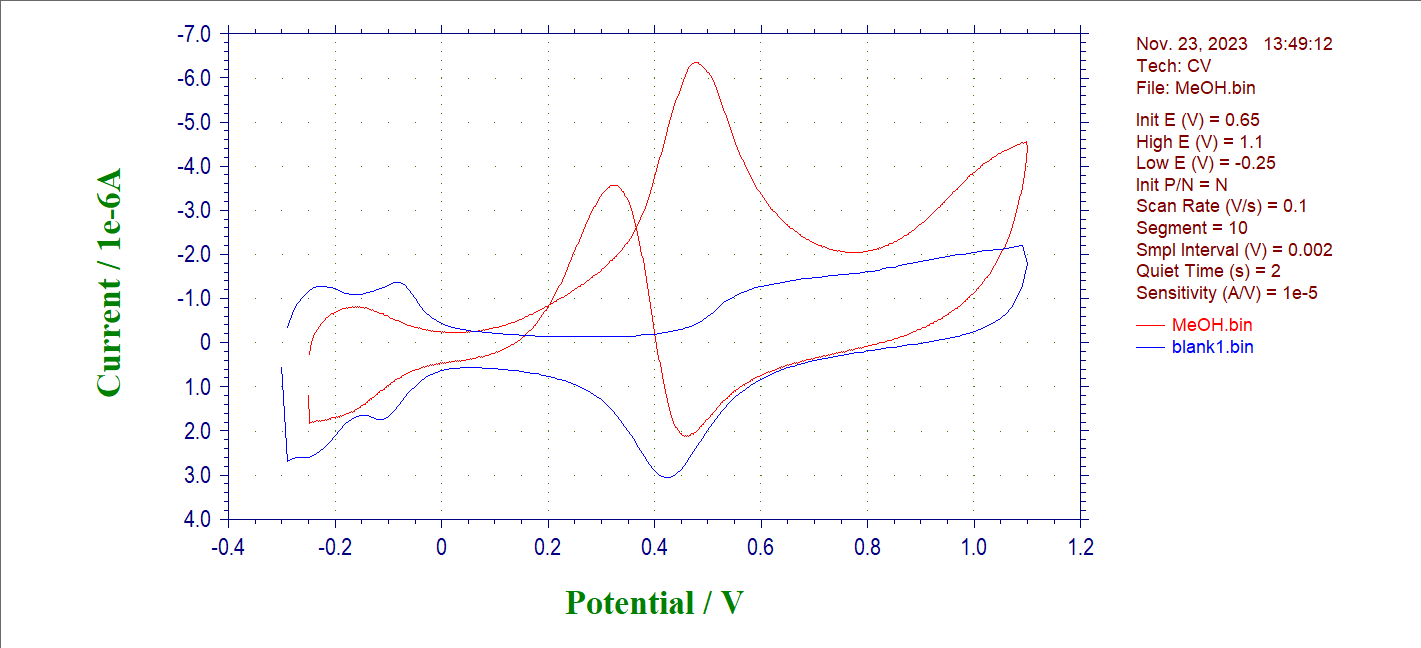
\includegraphics[width=.7\textwidth]{figures/3.png}
    \bicaption{$\ln\left(k/\mathrm{M}^{-1}\right)-\ln\left([\mathrm{H}^+]/\mathrm{M}\right)$ 图}{$\ln\left(k/\mathrm{M}^{-1}\right)-\ln\left([\mathrm{H}^+]/\mathrm{M}\right)$ diagram}
    \label{fig:3}
\end{figure}

拟合直线表达式为:
$$
\ln\left(k/\mathrm{M}^{-1}\right) = (1.92 \pm 0.12)\ln\left([\mathrm{H}^+]/\mathrm{M}\right) + (-9.35 \pm 0.17);\quad R^2 = 0.99642
$$

线性回归曲线的斜率即为反应级数,因此,反应对氢离子的级数为:
$$
n = (1.92 \pm 0.12) \approx 2
$$





